\begin{frame}{Clifford Tableau}{Structure}
    \vspace*{-3mm}
    Basically an expanded Check Matrix.
    \onslide<2->{
        \[
            \renewcommand{\arraystretch}{1.5}
            \left(
            \begin{array}{ccc|ccc|c}
                x_{1,1}      & \cdots & x_{1,n}      & z_{1,1}      & \cdots & z_{1,n}      & r_1      \\
                \vdots       & \ddots & \vdots       & \vdots       & \ddots & \vdots       & \vdots   \\
                x_{n,1}      & \cdots & x_{n,n}      & z_{n,1}      & \cdots & z_{n,n}      & r_n      \\
                \hline
                x_{(n+1),1}  & \cdots & x_{(n+1),n}  & z_{(n+1),1}  & \cdots & z_{(n+1),n}  & r_{n+1}  \\
                \vdots       & \ddots & \vdots       & \vdots       & \ddots & \vdots       & \vdots   \\
                x_{(2n),1}   & \cdots & x_{(2n),n}   & z_{(2n),1}   & \cdots & z_{(2n),n}   & r_{2n}   \\
                \hline
                x_{(2n+1),1} & \cdots & x_{(2n+1),n} & z_{(2n+1),1} & \cdots & z_{(2n+1),n} & r_{2n+1} \\
            \end{array}
            \right)
        \]
    }

    \fullfootcite{02_ImprovedSimulationOfStabilizerCircuits}
\end{frame}

\begin{frame}{Clifford Tableau}{Interpretation}
    Developers of the following algorithm introduce additional \(n\) "Destabilizer" generators,
    which are Pauli operators that together with the stabilizer generators generate the full Pauli group.

    \begin{minipage}{0.5\linewidth}
        \begin{itemize}
            \setlength{\itemsep}{0.25\baselineskip}
            \item
            \onslide<2->{
                Rows \(1\) to \(n\) represent Destabilizers.
            }
            \onslide<3->{
                \item
                Rows \(n+1\) to \(2n\) represent Stabilizers.
            }
            \onslide<4->{
                \item
                Row \(2n+1\) is scratch-space.
            }
            \onslide<5->{
                \item
                \(r_i\) of row \(i\) represents the global phase, \\
                \(r_i=0\) for \(+1\) and \(r_i=1\) for \(-1\).
            }
        \end{itemize}
    \end{minipage}%
    \begin{minipage}{0.5\linewidth}
        \onslide<2->{
            \begin{figure}
                \centering
                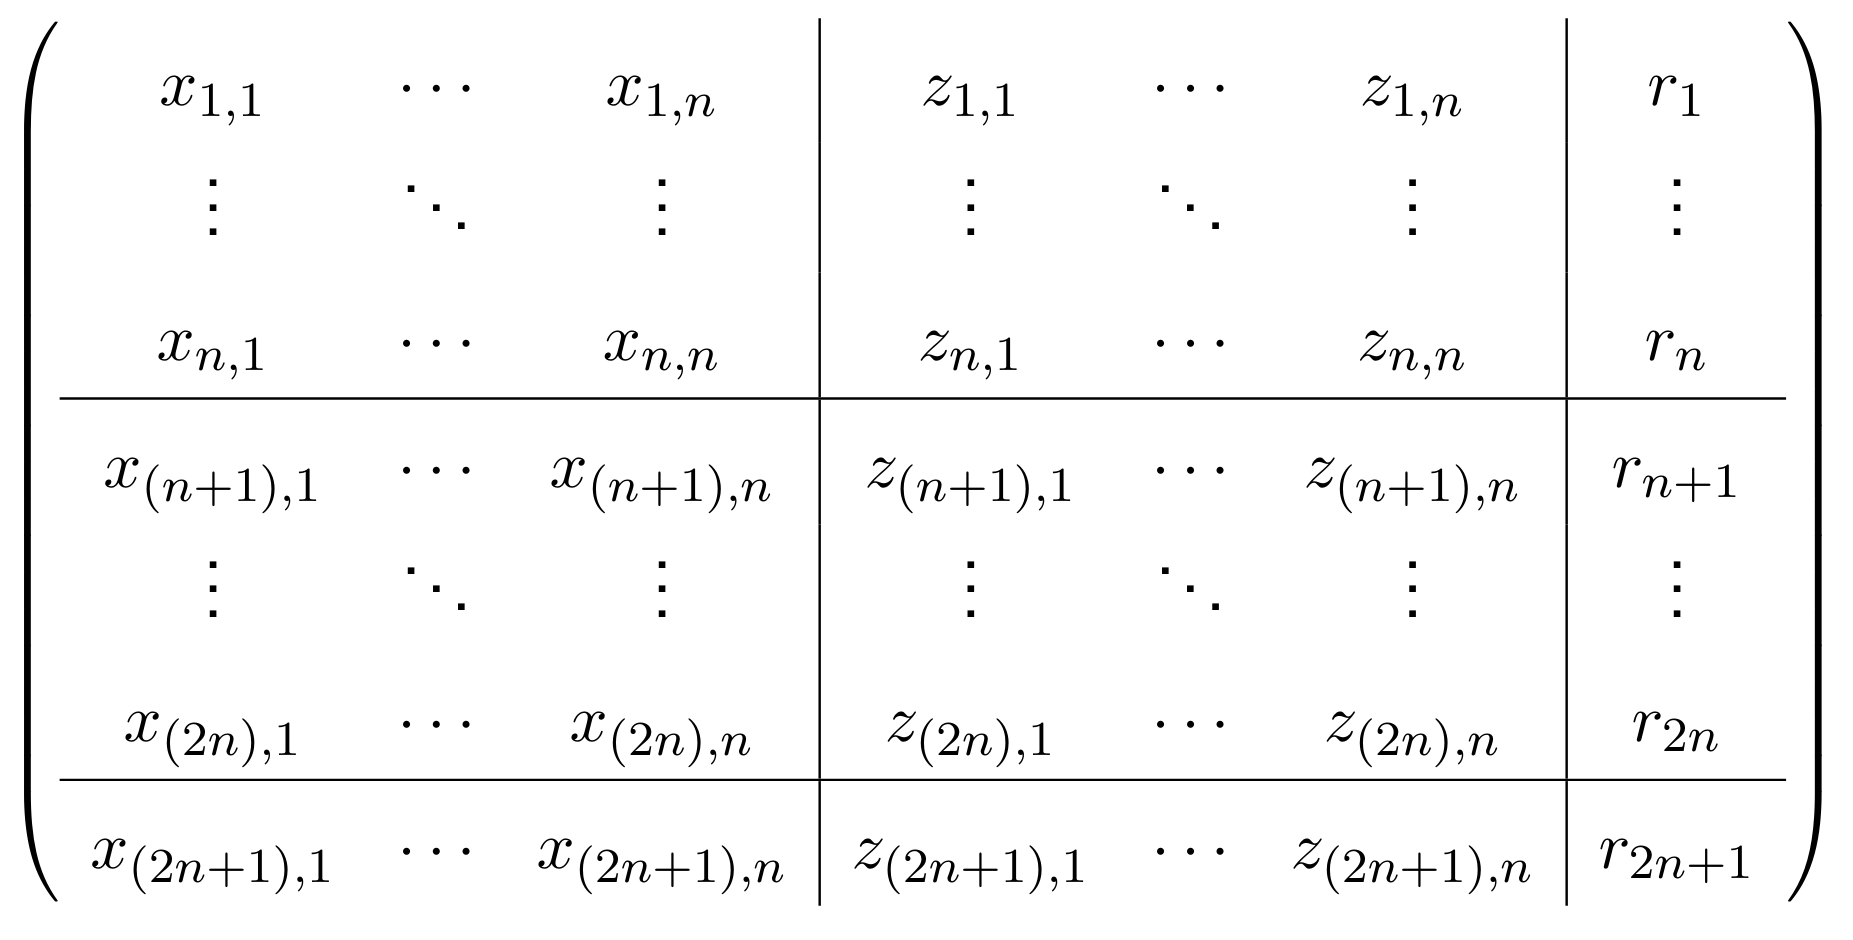
\includegraphics[scale=0.15]{images/CliffordTableau}
                \label{fig:clifford-tableau}
            \end{figure}
        }
    \end{minipage}

    \vspace*{5mm}

    \fullfootcite{02_ImprovedSimulationOfStabilizerCircuits}
\end{frame}


\begin{frame}{Clifford Tableau}{Initial Tableau}
    Pauli-\(Z\) gates stabilize \(\ket{0}\) states and Pauli-\(X\) gates destabilize \(\ket{0}\) states.

    \onslide<2->{
        \vspace*{2mm}
        \(\qquad\Longrightarrow\)
        Tableau for \(\ket{0}^{\otimes n}\) has an Identity submatrix for its first \((2n)\times(2n)\) submatrix.
    }
    \onslide<3->{
        \[
            \text{Tableau for }\ket{00}\text{ is }
            \left(
            \begin{array}{cc|cc|c}
                1 & 0 & 0 & 0 & 0 \\
                0 & 1 & 0 & 0 & 0 \\
                \hline
                0 & 0 & 1 & 0 & 0 \\
                0 & 0 & 0 & 1 & 0 \\
                \hline
                0 & 0 & 0 & 0 & 0 \\
            \end{array}
            \right)
        \]
    }

    \vspace*{15mm}

    \fullfootcite{02_ImprovedSimulationOfStabilizerCircuits}
\end{frame}
